\chapter{Aufbau des Helium-Neon-Lasers} \label{aufbau helium neon laser}

In diesem Versuch wird ein Helium-Neon-Laser (HeNe-Laser) selbstständig auf einer optischen Bank aufgebaut und justiert.

Für die Realisierung eines Lasers sind grundsätzlich drei Hauptkomponenten erforderlich:

\begin{itemize}
    \item Ein aktives Medium, das mindestens ein Drei-Niveau-System aufweist, um eine Besetzungsinversion ermöglichen zu können. 
    \item Eine optische Pumpe, die Energie zuführt, um die Besetzungsinversion im aktiven Medium zu erzeugen. 
    \item Ein optischer Resonator, der die stimulierte Emission unterstützt, die Wellenlänge selektiert und die Strahlrichtung bestimmt.
\end{itemize}

Das durch diesen Mechanismus erzeugte Laserlicht ist nahezu monochromatisch und weist eine hohe Kohärenz auf. 
Durch den optischen Resonator ist der Strahl stark gebündelt und erreicht eine hohe Intensität.

Im hier verwendeten Aufbau dient ein Gasgemisch aus Helium und Neon als aktives Medium, wobei das Verhältnis typischerweise etwa 10:1 zugunsten von Helium beträgt.


\FloatBarrier
\begin{figure}[htbp]
\centering
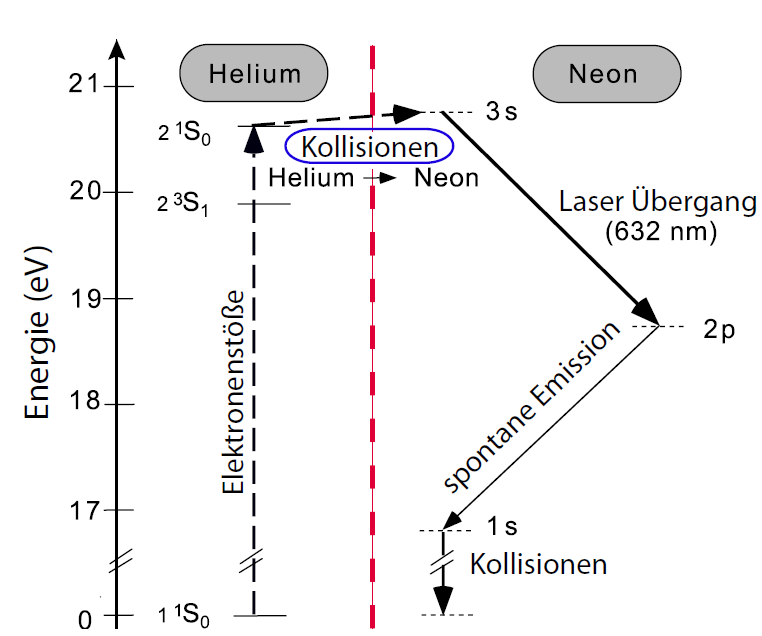
\includegraphics[width=1\linewidth]{Energielevel for He-Ne.png}
\caption{Energieleveldiagramm der Helium- und Neonatome. Der Energietransferprozess zur Erzeugung der Laserstrahlung ist schematisch dargestellt.\cite{praktikum}}
\label{fig:He-Ne}
\end{figure}
\FloatBarrier

Die notwendige Pumpenergie wird über eine elektrische Gasentladung bereitgestellt, welche Heliumatome in einen metastabilen angeregten Zustand versetzt. 
Die Energieniveaus dieser Zustände sind nahezu resonant mit dem 3s$_2$-Zustand der Neonatome (vgl. Abb. \ref{fig:He-Ne}). 
Durch inelastische Stoßprozesse kann so eine Energieübertragung erfolgen.

Befinden sich die Neonatome im 3s$_2$-Zustand, können sie durch stimulierte Emission in den 2p$_4$-Zustand übergehen. 
Dabei wird Licht mit einer charakteristischen Wellenlänge von 632,8 nm emittiert. 
Danach erfolgt eine spontane Emission zurück in den Grundzustand, wodurch der Prozess zyklisch abläuft.

Es existieren auch weitere Übergänge (z.B. im infraroten Bereich, siehe Abb.\ref{fig:Übergang}), die jedoch durch die Verwendung schmalbandiger Spiegel unterdrückt werden, da diese bevorzugt Licht im roten Spektralbereich reflektieren.

\FloatBarrier
\begin{figure}[htbp]
\centering
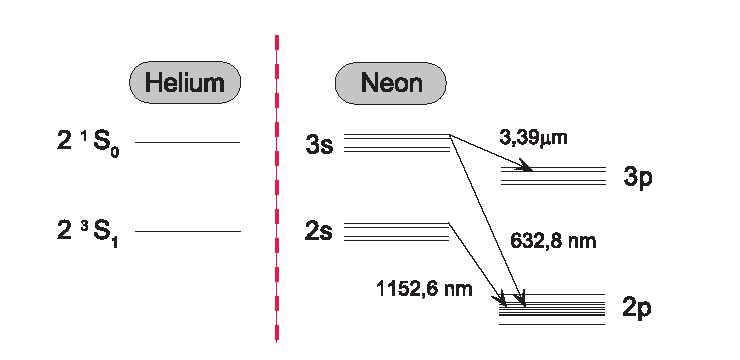
\includegraphics[width=1\linewidth]{mehrere Übergänge.png}
\caption{Weitere mögliche Übergänge im Neon-Atom.\cite{praktikum}}
\label{fig:Übergang}
\end{figure}
\FloatBarrier




\chapter{Justage des Helium-Neon-Lasers}


Der komplette Aufbau erfolgt auf einer optischen Bank und erfordert besondere Sorgfalt und Justiergenauigkeit.

Zunächst wird die optische Achse definiert. 
Dazu kommt ein zusätzlicher, externer Laser (Pilotlaser) zum Einsatz, um die Achse möglichst präzise zu justieren.

\begin{figure}[htbp]
    \centering
    \begin{minipage}[t]{0.48\textwidth}
        \centering
        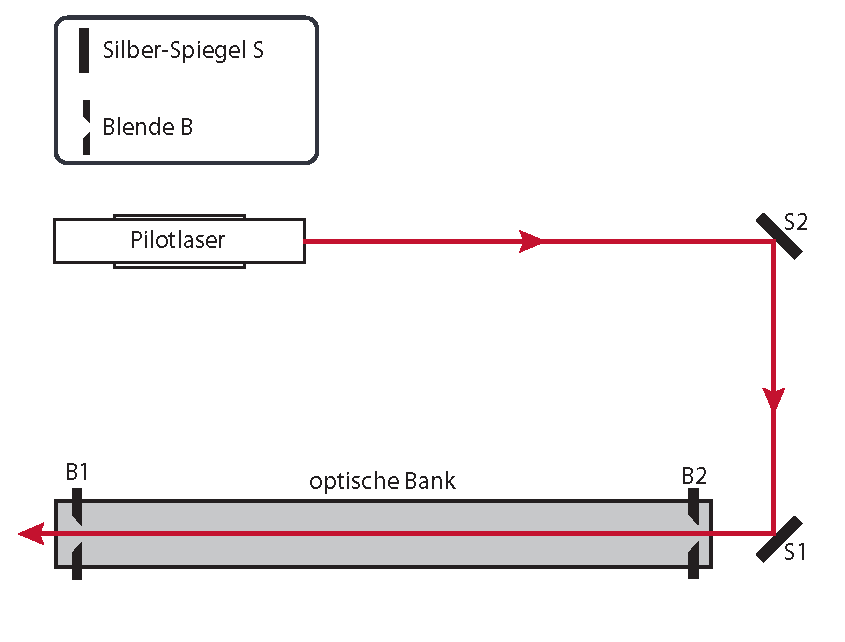
\includegraphics[width=\textwidth]{optische Achse.png}
       \caption{Justierung der optischen Achse mit Hilfe der Blenden.\cite{praktikum}}
        \label{fig:Blende}
    \end{minipage}
    \hfill
    \begin{minipage}[t]{0.48\textwidth}
        \centering
        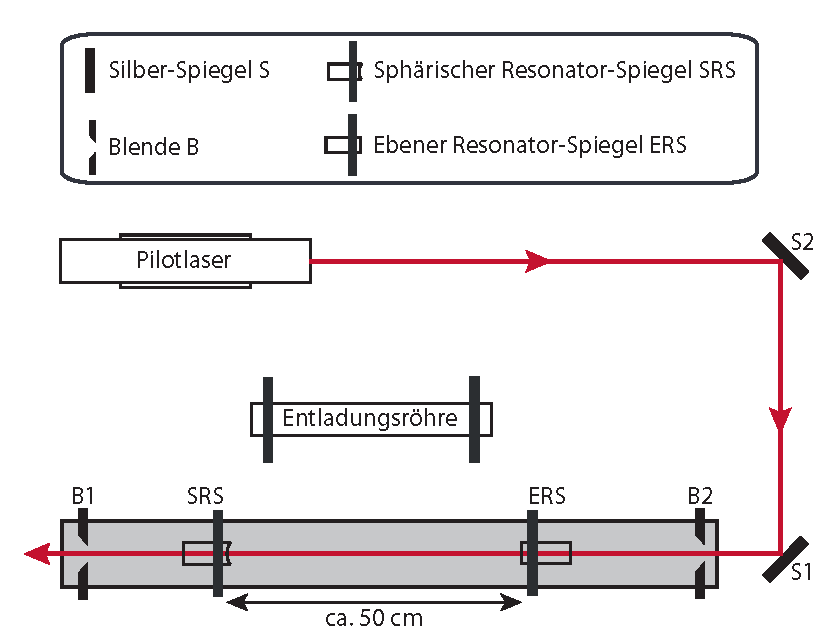
\includegraphics[width=\textwidth]{resonance spiegel.png}
        \caption{Justage der Resonatorspiegel.\cite{praktikum}}
        \label{fig:Spiegel}
   \end{minipage}
\end{figure}

Zuerst wird die Blende auf der optischen Achse ausgerichtet (Abb. \ref{fig:Blende}). 
Anschließend wird die Entladungsröhre eingebaut und so positioniert, dass möglichst wenig Licht innerhalb der Röhre verloren geht.
Danach erfolgt die Justage der Resonatorspiegel (einer sphärisch, einer planspiegelnd, halbdurchlässig), zunächst ohne Röhre. 
Ziel ist es, dass keine Reflexe mehr an der Wand sichtbar sind (vgl. Abb. \ref{fig:Spiegel}). 
Sobald dies erreicht ist, wird der Pilotlaser entfernt und die Entladungsröhre aktiviert. 
Durch feine Justierung der Spiegel sollte der Laser schließlich sichtbar aufblitzen – der Laser ist nun aktiv.



\chapter{Bestimmung der Wellenlänge}

Zur Wellenlängenbestimmung wird ein optisches Gitter außerhalb des Resonators hinter dem halbdurchlässigen Spiegel angebracht. 
Der Abstand der Interferenzmaxima kann dann über die Gleichungen \cite{Gitterformel}
\begin{centering}
\begin{itemize}
    \item [] $\tan(\alpha_i) = \frac{d_i}{a},$
    \item [] $\sin(\alpha_i) = \frac{\delta}{g}; \qquad \text{mit} \qquad \delta = i \cdot \lambda,$
    \item [] $\Rightarrow \lambda = \frac{\sin\big(\arctan\big(\frac{d_i}{a}\big)\big)}{i \cdot g} \label{eq:Wellenlänge},$
    \item []  $\Delta \lambda = \frac{1}{i \cdot g} \cdot \frac{1}{(d_i^2 + a^2)^\frac{3}{2}} \cdot \sqrt{(a^2 \cdot \Delta d)^2 + (da \cdot \Delta a
    )^2},$
\end{itemize}
\end{centering}

berechnet werden.
Mit der Gitterkonstanten $g = 600$ lines/mm und den gemessenen Werten ergibt sich folgende Tabelle:

\begin{table}[htbp]
    \centering
    \begin{tabular}{c|c|c|c}
        Ordnung & \(d_i ~[\text{m}]\) & \(a ~[\text{m}]\) & \(\lambda~[\text{nm}]\)\\
        \hline 
        -1 & 0,823 \(\pm\) 0,006 & 1,964 \(\pm\) 0,006 & 644,14 \(\pm\) 4,70 \\
        1 & 0,824 \(\pm\) 0,006 & 1,964 \(\pm\) 0,006 & 644,80 \(\pm\) 4,70 \\
    \end{tabular}
    \caption{Ermittelte Wellenlängen aus der ersten und negativen Ordnung.}
    \label{tab:Wellenlänge}
\end{table}


Der Mittelwert ergibt sich zu \(\lambda = (644,47 \pm 3,32)\)nm, was rund 1,8\% vom Literaturwert von 632,8 nm abweicht. 
Diese Differenz liegt außerhalb des angegebenen Fehlerbereichs und könnte auf eine fehlerhafte Gitterkonstante, nicht orthogonale Ausrichtung des Gitters oder auf eine systematische Fehlablesung zurückzuführen sein.


\chapter{Untersuchung der Polarisation}

Da das Laserlicht durch spontane Emission in alle Polarisationsrichtungen emittiert wird, wurde versucht, durch den Einsatz von Brewster-Fenstern eine Linearpolarisation zu erzwingen. 
Dabei nutzt man den Brewster-Winkel, bei dem Licht mit einer bestimmten Polarisationsrichtung bevorzugt transmittiert wird, während der orthogonal polarisierte Anteil reflektiert wird. 
Durch die Aneinanderreihung mehrerer Brewster-Fenster soll somit ein möglichst hoher Anteil linear polarisierten Lichts erzeugt werden.


Zur Untersuchung des Polarisationszustands wurde ein Polarisator in den Strahlengang eingebaut und die Intensität des transmittierten Lichts mit einer langsamen Photodiode gemessen (siehe Abb.~\ref{fig:Polar}).


\begin{figure}[H]
    \centering
    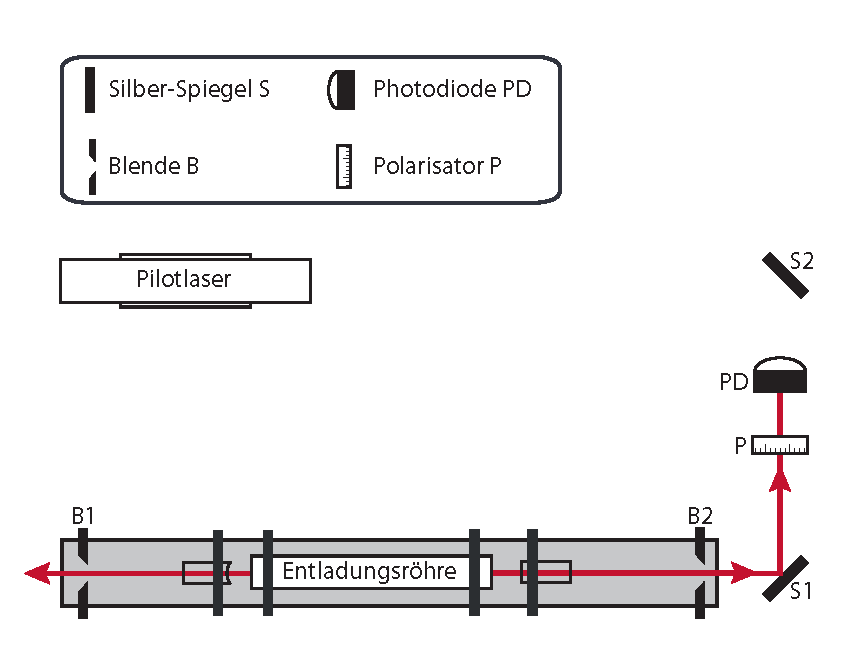
\includegraphics[width=0.5\linewidth]{Polarisation.png}
    \caption{Versuchsaufbau zur Untersuchung der Polarisation des Laserlichts\cite{praktikum}}
   \label{fig:Polar}
\end{figure}

Die Spannung, die proportional zur Intensität ist, wurde in Abhängigkeit vom Polarisationswinkel gemessen. 
Ein vorgeschalteter $50~\Omega$-Widerstand wurde verwendet, um den Stromfluss zu vergrößern und die Messung zu erleichtern. 
Die gemessenen Werte sind in Tabelle~\ref{tab:Wellenlaenge} dargestellt.

\begin{table}[htbp]
    \centering
    \begin{tabular}{c|c}
        Winkel \(~[\text{°}]\) & Spannung \(U~[\text{mV}]\) \\
        \hline
        0 \(\pm\) 1 & 10 \(\pm\) 1{,}5 \\
        20 \(\pm\) 1 & 1{,}75 \(\pm\) 0{,}3 \\
        40 \(\pm\) 1 & 2 \(\pm\) 0{,}5 \\
        60 \(\pm\) 1 & 2{,}2 \(\pm\) 0{,}5 \\
        80 \(\pm\) 1 & 11{,}5 \(\pm\) 1 \\
        100 \(\pm\) 1 & 21 \(\pm\) 2 \\
        120 \(\pm\) 1 & 27{,}5 \(\pm\) 3 \\
        140 \(\pm\) 1 & 25 \(\pm\) 3 \\
        160 \(\pm\) 1 & 17 \(\pm\) 2 \\
        180 \(\pm\) 1 & 7{,}5 \(\pm\) 1 \\
        200 \(\pm\) 1 & 0{,}9 \(\pm\) 0{,}3 \\
        220 \(\pm\) 1 & 1{,}7 \(\pm\) 0{,}3 \\
        240 \(\pm\) 1 & 2{,}8 \(\pm\) 0{,}35 \\
        260 \(\pm\) 1 & 11 \(\pm\) 1 \\
        280 \(\pm\) 1 & 18 \(\pm\) 1{,}5 \\
        300 \(\pm\) 1 & 24 \(\pm\) 2 \\
        320 \(\pm\) 1 & 21 \(\pm\) 2 \\
        340 \(\pm\) 1 & 13 \(\pm\) 1{,}5 \\
    \end{tabular}
    \caption{Gemessene Spannungen bei unterschiedlichen Polarisationswinkeln}
    \label{tab:Wellenlaenge}
\end{table}

Da der Laser annähernd linear polarisiert ist, kann der Verlauf der Intensität in Abhängigkeit vom Polarisationswinkel durch das \textbf{Malus’sche Gesetz} \cite{Malus} beschrieben werden:

\begin{equation*}
    I = I_0 \cdot \cos^2(\theta - \theta_0) + b .
\end{equation*}

Hierbei ist $I_0$ die maximale Intensität, $\theta_0$ der Winkel der Polarisationsebene und $b$ ein Offset (z.\,B. durch Umgebungslicht oder systematische Messfehler).

\begin{table}[htbp]
    \centering
    \begin{tabular}{c|c}
        Parameter & Wert \\
        \hline
        $U_0$ & (21{,}59 \(\pm\) 0{,}79) mV \\
        $\theta_0$ & (125{,}97 \(\pm\) 0{,}64) ° \\
        $b$ & (0{,}22 \(\pm\) 0{,}17) mV \\
    \end{tabular}
    \caption{Angepasste Parameter zur Beschreibung der Polarisation}
    \label{tab:WertePol}
\end{table}

Die zugehörige Ausgleichskurve ist in Abbildung~\ref{fig:PolarisationFigur} dargestellt.

\begin{figure}[H]
    \centering
    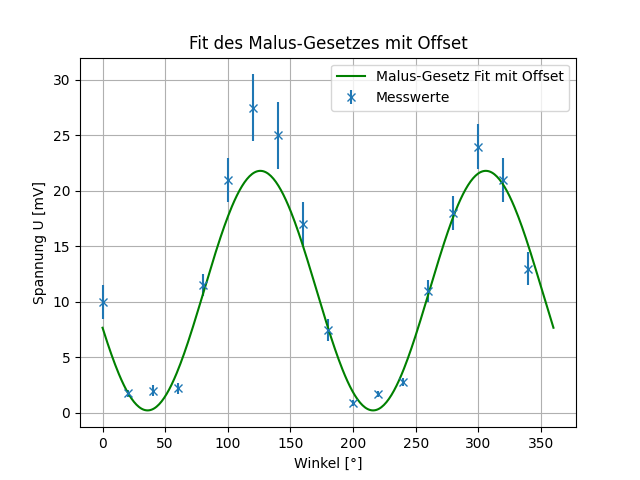
\includegraphics[width=0.5\linewidth]{Figure_2}
    \caption{Fit des Malus’schen Gesetzes an die Messwerte ($\chi^2_\text{red} = 5{,}16$)}
    \label{fig:PolarisationFigur}
\end{figure}

Es ist erkennbar, dass die Messwerte nicht vollständig mit dem Fit übereinstimmen.
Die reduzierte Chi-Quadrat-Abweichung $\chi^2_\text{red} = 5{,}16$ zeigt, dass der Fit nicht ideal ist, jedoch noch im akzeptablen Bereich liegt. 
Zusätzlich wurde eine Intensität ohne Polarisator von $I_0 = (33 \pm 1{,}5)~\text{mV}$ gemessen.

Die Abweichungen lassen sich durch verschiedene systematische Fehler erklären:

\begin{itemize}
    \item Der Polarisator war möglicherweise nicht korrekt ausgerichtet oder hatte interne Spannungen, die zu Doppelbrechung führen.
    \item Rückreflexionen oder Streulicht könnten das Messergebnis verfälscht haben.
    \item Die Intensitätsmessung war möglicherweise nicht vollständig stabil, sodass es zu Schwankungen kam.
\end{itemize}

Trotz der genannten Unstimmigkeiten lässt sich erkennen, dass die gemessenen Spannungen in guter Näherung dem Verlauf eines $\cos^2$-Gesetzes folgen, was das Malus’sche Gesetz bestätigt.

Der Polarisationsgrad \( PG \) des Lasers lässt sich aus den Fit-Parametern wie folgt berechnen \cite{praktikum}:
\begin{equation*}
    PG = \frac{U_\text{max} - U_\text{min}}{U_\text{max} + U_\text{min}} = \frac{U_0 - b}{U_0 + b} = 0{,}98 \pm 0{,}01.
\end{equation*}

Da der Polarisationsgrad kleiner als 1 ist, lässt sich daraus schließen, dass das Laserlicht nicht vollständig linear polarisiert ist. 
Ein geringer zirkular oder elliptisch polarisierter Anteil ist vorhanden. 
Dies ist zu erwarten, da die Brewster-Fenster nicht ideal sind und eine perfekte Polarisierung unter realen Bedingungen nicht erreicht werden kann.

\chapter{Messung des Strahlprofils}

In diesem Versuchsteil soll das Strahlprofil innerhalb des Resonators untersucht werden. 
Hierzu wird eine verstellbare Spaltblende (Messschieber) senkrecht zur Strahlachse montiert, sodass sie entlang der Querachse des Strahls verschoben werden kann. 
Auf diese Weise lässt sich die kritische Breite des Laserstrahls \( d(z) \) in Abhängigkeit von der Position \( z \) entlang des Strahlengangs bestimmen.

Durch schrittweise Verkleinerung der Spaltbreite wird der Strahl zunehmend beschnitten, was zu Verlusten im Resonator führt. 
Sobald diese Verluste größer sind als die Verstärkung im Lasermedium, bricht die Laseremission ab. 
Die kritische Spaltbreite hängt daher direkt vom lokalen Strahldurchmesser ab.

Das Strahlprofil eines idealen transversalen Grundmodus (TEM\textsubscript{00}) eines Gauß-Strahls folgt der bekannten Form \cite{praktikum} :

\begin{equation*}
    w(z) = w_0 \cdot \sqrt{1+\left(\frac{z}{z_R}\right)^2}
\end{equation*}
 
mit einem Minimum der Strahlweite \( w_0 \) an der Stelle \( z = 0 \), der sogenannten Strahltaille. Für einen halbsymmetrischen Resonator mit einem planen und einem sphärischen Spiegel ergibt sich die theoretische Taille \( w_0 \) aus \cite{praktikum}:

\begin{equation*}
    w_0 = \sqrt{\frac{\lambda}{\pi} \cdot \sqrt{L \cdot (R - L)}}
\end{equation*}

wobei \( L \) die Resonatorlänge (Abstand der Spiegel) und \( R \) der Krümmungsradius des sphärischen Spiegels ist. Die zugehörige Rayleigh-Länge ergibt sich zu:

\begin{equation*}
    z_R = \frac{\pi w_0^2}{\lambda}.
\end{equation*}

Da sich die Strahltaille bei einem halbsymmetrischen Resonator nahe am planen Spiegel befindet, wird die Position \( z = 0 \) auf diesen Punkt bezogen.

Zur Auswertung der Messdaten wurde die Form des Gaußstrahlradius

\begin{equation*}
    w(z) = d_0 \cdot \sqrt{1+\left(\frac{z}{z_R}\right)^2}
\end{equation*}

durch nichtlineare Regression an die experimentellen Daten angepasst. 
Dabei ist zu beachten, dass die gemessene kritische Spaltbreite \( d(z) \) nicht dem theoretischen Strahldurchmesser \( 2w(z) \) entspricht, sondern nur proportional dazu ist. Dieser Zusammenhang \cite{praktikum} wird durch eine Proportionalitätskonstante \( c \) beschrieben:

\begin{equation}
    2 \cdot w(z) = c \cdot d(z)
    \label{eq:proportionalitaet}
\end{equation}

Die folgenden Tabellen zeigen die gemessenen Werte der kritischen Spaltbreite \( d(z) \) in Abhängigkeit von der Position \( z \) für zwei unterschiedliche Resonatorlängen:

\begin{table}[htbp]
    \centering
    \begin{tabular}{S[table-format=1.2(2)]|S[table-format=3.0(1)]}
        {$d(z)\,\si{\milli\meter}$} & {$z\,\si{\milli\meter}$} \\
        \hline
        1.35 \pm 0.01 & 3 \pm 1 \\
        2.20 \pm 0.01 & 401 \pm 1 \\
        2.25 \pm 0.01 & 415 \pm 1 \\
        2.50 \pm 0.01 & 445 \pm 1 \\
        2.60 \pm 0.01 & 487 \pm 1 \\
        2.70 \pm 0.01 & 505 \pm 1 \\
    \end{tabular}
    \caption{Messung des Strahlprofils bei einer Resonatorlänge von \SI{62.0}{\centi\meter}}
    \label{tab:62}
\end{table}

\begin{table}[htbp]
    \centering
    \begin{tabular}{S[table-format=1.2(2)]|S[table-format=3.0(1)]}
        {$d(z)\,\si{\milli\meter}$} & {$z\,\si{\milli\meter}$} \\
        \hline
        1.90 \pm 0.01 & 12 \pm 1 \\
        3.80 \pm 0.01 & 506 \pm 1 \\
        4.90 \pm 0.01 & 555 \pm 1 \\
        5.85 \pm 0.01 & 635 \pm 1 \\
    \end{tabular}
    \caption{Messung des Strahlprofils bei einer Resonatorlänge von \SI{76.3}{\centi\meter}}
    \label{tab:76_3}
\end{table}

Die durch Ausgleichsrechnung bestimmten Parameter sowie die theoretischen Vergleichswerte sind in Tabelle~\ref{tab:BStrahl} zusammengefasst:

\begin{table}[htbp]
    \centering
    \begin{tabular}{S|S|S|S|S|S}
        {$L\,\si{\centi\meter}$} & {$d_0\,\si{\micro\meter}$} & {$z_R\,\si{\centi\meter}$} &
        {$w_{0,\text{theo}}\,\si{\micro\meter}$} & {$z_{R,\text{theo}}\,\si{\centi\meter}$} & {$c$} \\
        \hline
        62.0 \pm 0.3 & 1332 \pm 49 & 29.15 \pm 1.56 & 312 & 48.54 & 0.469 \pm 0.017 \\
        76.3 \pm 0.3 & 1831 \pm 50 & 24.67 \pm 0.82 & 292 & 42.52 & 0.319 \pm 0.009 \\
    \end{tabular}
    \caption{Experimentell bestimmte und theoretisch berechnete Strahlparameter}
    \label{tab:BStrahl}
\end{table}

Die zugehörigen Ausgleichskurven sind in den folgenden Abbildungen dargestellt:

\begin{figure}[htbp]
    \centering
    \begin{subfigure}[t]{0.48\textwidth}
        \centering
        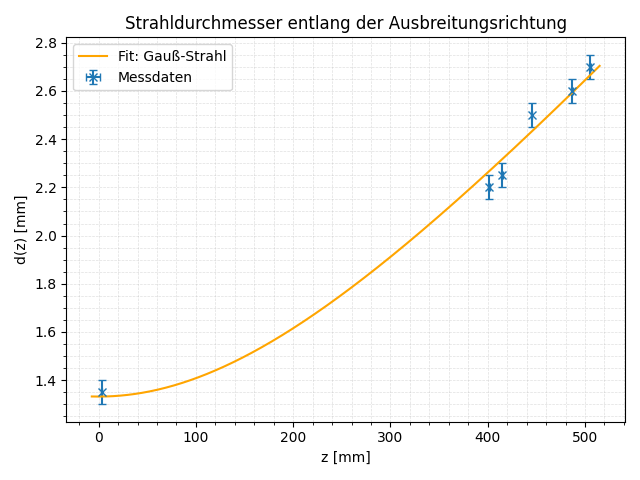
\includegraphics[width=\textwidth]{Figure_3.png}
        \caption{Strahlprofil für \(L = \SI{62.0}{\centi\meter}\), \(\chi^2 = 1{,}52\)}
        \label{fig:62}
    \end{subfigure}
    \hfill
    \begin{subfigure}[t]{0.48\textwidth}
        \centering
        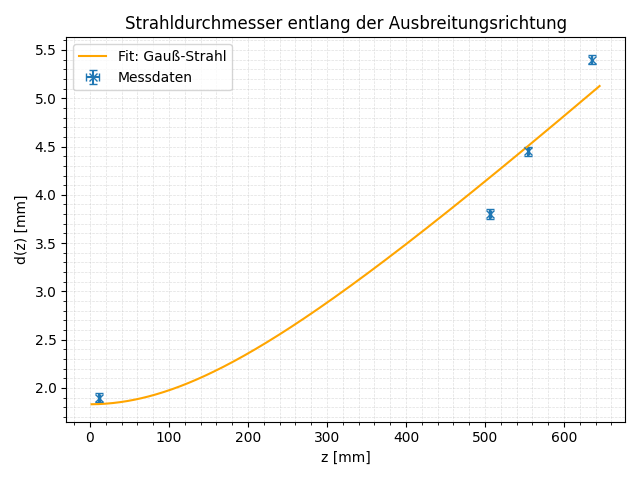
\includegraphics[width=\textwidth]{Figure_4.png}
        \caption{Strahlprofil für \(L = \SI{76.3}{\centi\meter}\), \(\chi^2 = 53{,}80\)}
        \label{fig:76}
    \end{subfigure}
    \caption{Gemessene Strahlprofile mit Fitkurven}
\end{figure}

Die Anpassung bei \(L = \SI{62.0}{\centi\meter}\) gelingt deutlich besser als bei \(L = \SI{76.3}{\centi\meter}\), was sich auch im stark erhöhten \(\chi^2\)-Wert für den zweiten Fall widerspiegelt. 
Ursachen hierfür könnten die geringere Anzahl an Messpunkten sowie experimentelle Schwierigkeiten beim Ansetzen der Spaltblende sein, insbesondere bei größeren Spaltweiten, bei denen der Laser noch nicht vollständig erlischt.

Ein Vergleich der experimentell bestimmten Rayleigh-Längen mit den theoretisch erwarteten Werten zeigt eine Abweichung von etwa 40\,\%. 
Diese Diskrepanz könnte durch systematische Fehler bei der Ablesung sowie durch eine fehlerhafte Ausrichtung der Spaltblende verursacht sein: 
Ist diese nicht exakt senkrecht zur Strahlachse positioniert, erscheint die effektive Spaltbreite kleiner, was zu einer Überschätzung des Strahldurchmessers führt.

Zudem ist zu beachten, dass die gemessene Spaltbreite nicht direkt dem \SI{1}{/e^2}-Durchmesser des Laserstrahls entspricht. 
Der Strahlradius \( w(z) \) beschreibt den Abstand von der Strahlachse, bei dem die Intensität auf \( 1/e^2 \) ihres Maximalwertes abgesunken ist. 
Die Abschattung durch die Blende führt jedoch bereits bei größerer Intensität zu einem Erlöschen der Emission.

Aus diesem Grund wurde eine Proportionalitätskonstante \( c \) eingeführt, um den Zusammenhang zwischen dem theoretischen Strahldurchmesser und der experimentell bestimmten kritischen Spaltbreite herzustellen. 
Diese Beziehung ist in Gleichung~\eqref{suchung_c} gegeben:

\begin{equation}
    2 \cdot w(z) = c \cdot d(z)
    \label{suchung_c}
\end{equation}

Der Mittelwert der ermittelten Proportionalitätskonstanten beträgt:

\begin{equation*}
    c = 0{,}394 \pm 0{,}008
\end{equation*}

Damit lässt sich die kritische Spaltbreite in einen effektiven Strahldurchmesser überführen. 
Diese Konstante stellt somit eine zentrale experimentelle Größe dar, die den Abgleich zwischen theoretischem Modell und praktischer Messung ermöglicht.